\chapter{实现}

\section{Schedule}

不能支持嵌套task,用pre yield变量来控制。

\section{内存}

从初始化顺序上来看,分为hugepage初始化之前和之后。初始化后才能用hugepage相关接口。

提供什么接口,三种生命周期范围、持久性:
\begin{easylist}[itemize]
    & 常驻
    & session
    & IO
\end{easylist}

使用场景
\begin{easylist}[itemize]
    & core private memory
    & sche\_task
    & RDMA
    & buffer\_t
    && libnvme
    & little object
    & ring
\end{easylist}

采用buddy算法管理连续内存分配

动态化

用面向对象的方式处理,每个core对应一个MR对象。public的也是如此。

每个对象内嵌一个buddy对象管理hugepage的分配、释放。
另外,从core的MR里,利用buddy算法分配连续内存,用于ring等小对象。

禁止在一个core内malloc,由另外一个core进行free。

怎么抽象一般内存和hugepage-based内存?

抽象出head,core和public重用代码。第一选择head,第二执行head的操作。

\subsection{buffer}

\begin{center}
    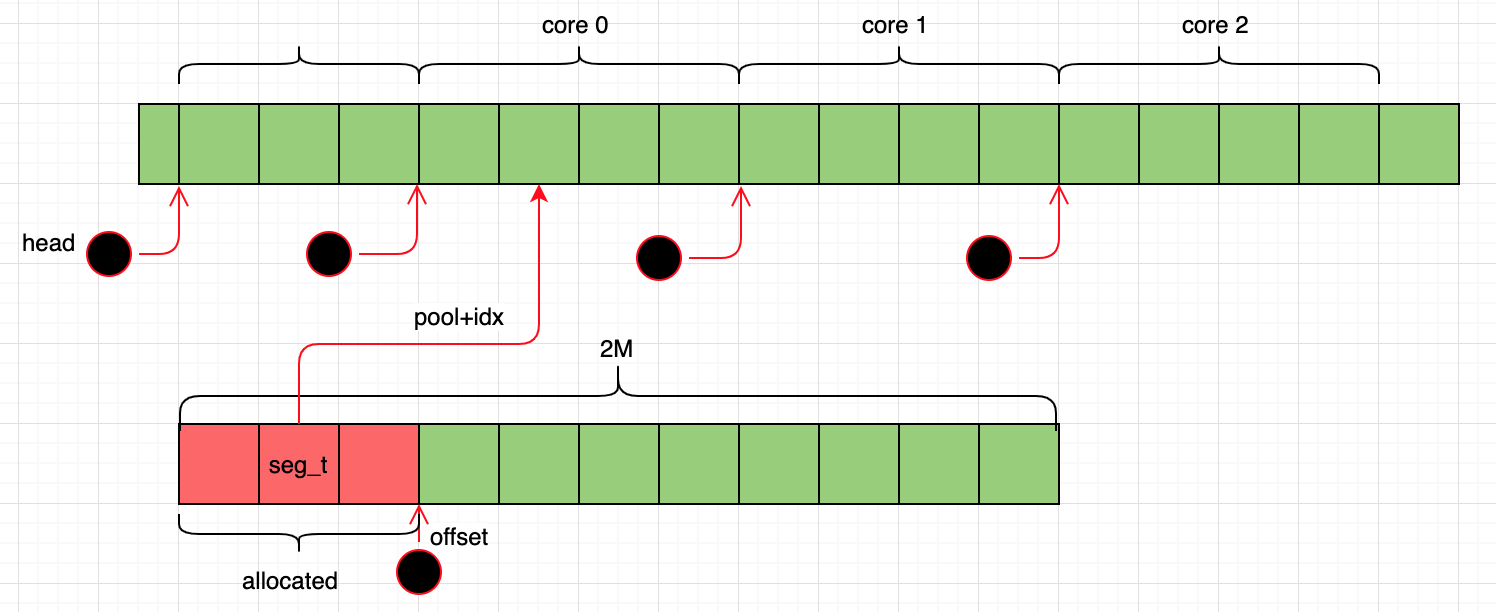
\includegraphics[width=10cm]{../imgs/buffer-t.png}
\end{center}

每个内存区域的\hl{第一个hugepage用来保存该区域的元数据信息},可供分配的是后面的hugepages。
在元数据信息中加上buddy,可用来支持buddy算法。

buffer的每个seg都包含有虚拟地址和物理地址。

\subsection{Memory Pool}

\begin{center}
    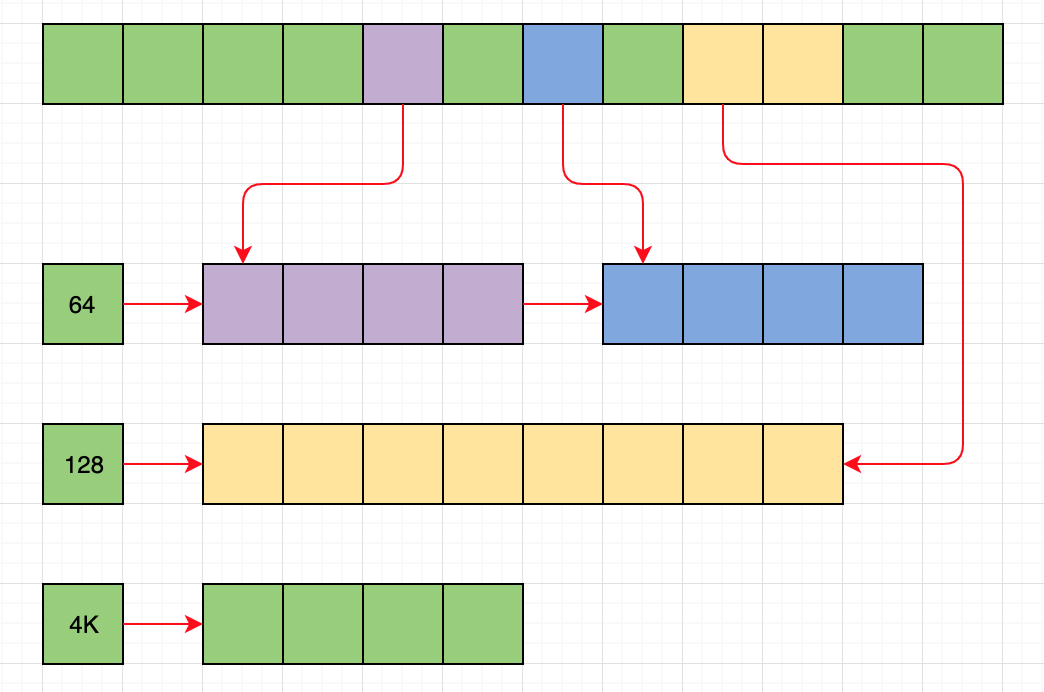
\includegraphics[width=10cm]{../imgs/memory-pool.png}
\end{center}

直接从hugepage申请内存,从hugepage申请一个hugepage,用于小对象。pool管理多个size的小对象队列。
根据要malloc的size,定位到队列。

free时按指针查找属于哪个hugepage。每个hugepge对应起始地址和结束地址以及所在队列的标识。
这样可以保留malloc和free的语法和语义。

hugepage层只需要提供分配单个hugepage的接口,一个队列可以由一个或多个hugepage构成。

或者,memory pool按4k进行组织,同样采用buddy算法。在其上实现ring等。

\hl{每layer都要动态化,包括增和减}。

\subsection{NVMe}

NVMe为什么需要物理地址?

direct io需要512对齐。

\subsection{RDMA}

每个连接$1024*512$内存。

\subsection{IO}

\begin{center}
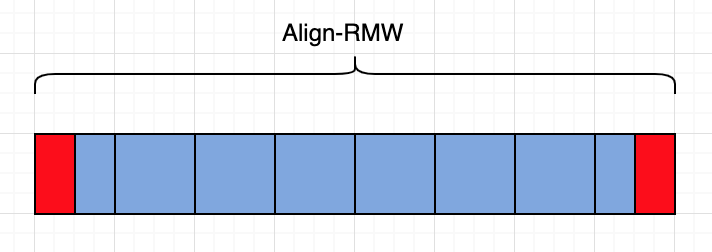
\includegraphics[width=10cm]{../imgs/io-align.png}
\end{center}

首尾页对齐

buffer\_t包含一个seg时,方便处理。如果有多个seg,是否需要分配连续的大块内存。

\hl{SPDK的大IO问题}:NVMe需要物理内存,并且一次io物理内存是连续的。
malloc的内存,不容易找到物理内存。
2M的hugepage虽然能获取虚拟地址连续的4M地址空间,但底层物理内存未必连续。
用1G的hugepage更容易管理。

GFM的机制是什么?barrier去解决RMW、chunk恢复等问题?

\section{Disk}

\begin{center}
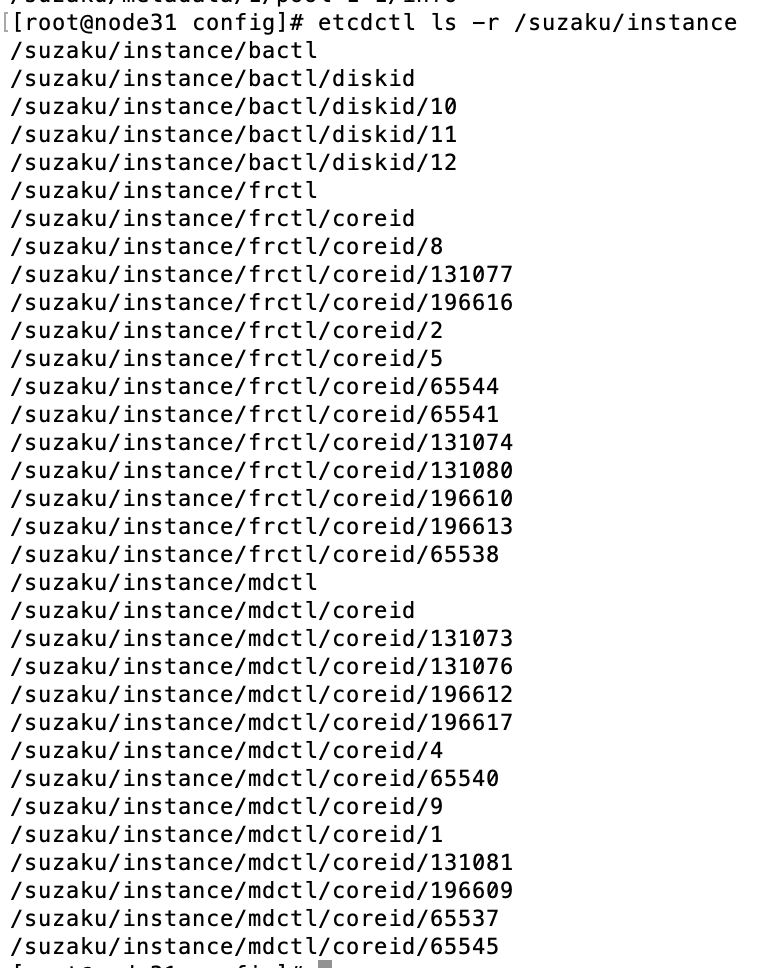
\includegraphics[width=10cm]{../imgs/etcd-suzaku-instance.png}
\end{center}

通过独立线程scan到各个disk,放入slot中。并注册到etcd。

\begin{center}
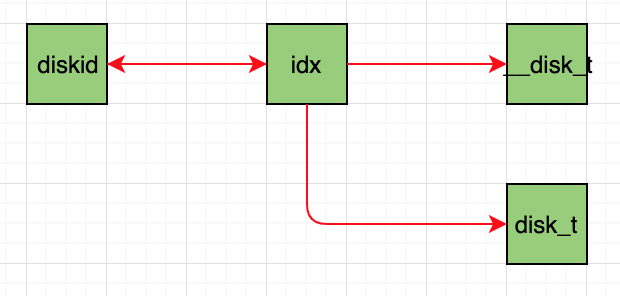
\includegraphics[width=10cm]{../imgs/diskid-slot.png}
\end{center}

全局唯一的diskid放在etcd上。根据diskid查找到slot idx。根据slot idx索引到disk。
即可执行IO操作。
